\documentclass{beamer}

\usepackage[utf8]{inputenc}
\usepackage[T1]{fontenc}
\usepackage[ngerman]{babel}
\usepackage{graphicx} % Bilder
\usepackage{wrapfig} % Umflussbilder
\usepackage{multicol} % Multiple columns
\usepackage{minted} % Haskell source code
\usepackage{framed} % Frames around source code
\usepackage[framemethod=tikz]{mdframed} % Frames
\usepackage{verbatim} % \begin{comment}...\end{comment}
\usepackage{etoolbox} % manipulate minted
\AtBeginEnvironment{minted}{\fontsize{10}{10}\selectfont}
\AfterEndEnvironment{minted}{}

\mdfdefinestyle{fancy}{
  roundcorner=5pt,
  linewidth=4pt,
  linecolor=red!80,
  backgroundcolor=red!20
}
\newmdenv[style=fancy]{important}

% redifine \em for \emph to use bold instead of italics
\makeatletter
\DeclareRobustCommand{\em}{%
  \@nomath\em \if b\expandafter\@car\f@series\@nil
  \normalfont \else \bfseries \fi}
\makeatother

% Stuff for Beamer
\beamertemplatenavigationsymbolsempty
\usetheme{Warsaw}

\title{Fortgeschrittene Funktionale Programmierung in Haskell}

\begin{document}
  
%----------------------------------------------------------------------------------------  

  \begin{frame}
  \begin{center}
    \huge\textbf{Fortgeschrittene Funktionale Programmierung in Haskell}\\ \bigskip
    \LARGE Universität Bielefeld, Sommersemester 2015\\ \bigskip
    \large Jonas Betzendahl \& Stefan Dresselhaus
    \end{center}
  \end{frame}

%----------------------------------------------------------------------------------------  
\begin{frame}[allowframebreaks]{Outline}
\vfill
Übersicht für Heute:\smallskip

\tableofcontents
\end{frame}

\section{Wiederholung}

%----------------------------------------------------------------------------------------

\begin{frame}

\begin{center}
\Large
\textbf{Wiederholung}
\end{center}

\end{frame}

%----------------------------------------------------------------------------------------

\begin{frame}

\textbf{Leseempfehlung:}

\begin{center}
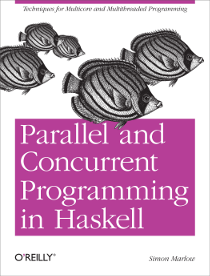
\includegraphics[scale=0.5]{../Woche6/parcur.png} 
\end{center}
\pause

\dots srsly!

\end{frame}

%----------------------------------------------------------------------------------------

\begin{frame}

\begin{center}
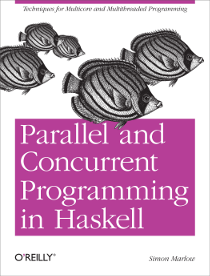
\includegraphics[scale=1]{../Woche6/parcur.png} 
\end{center}

\end{frame}

%----------------------------------------------------------------------------------------

\begin{frame}

\textbf{Überblick:}
\pause

\begin{multicols}{2}
\textbf{Parallelism:}
\begin{itemize}
\item Mehrere Hardwareelemente\pause
\item Antwort schneller kriegen\pause
\item deterministisch (i.d.R.)\pause
\item oft deklarativ\pause
\end{itemize}
\columnbreak
\textbf{Concurrency:}
\begin{itemize}
\item Mehrere Threads\pause
\item Dinge gleichzeitig tun\pause
\item nichtdeterministisch\pause
\item oft impertativ
\end{itemize}
\end{multicols}

\end{frame}

%----------------------------------------------------------------------------------------

%----------------------------------------------------------------------------------------

\section{Threads, MVars, etc.}

\begin{frame}

\begin{center}
\Large
\textbf{Die Basics: Threads, MVars, etc.}
\end{center}

\end{frame}

%----------------------------------------------------------------------------------------

\section{Software Transactional Memory}

\begin{frame}

\begin{center}
\Large
\textbf{Software Transactional Memory (STM)}
\end{center}

\end{frame}

%----------------------------------------------------------------------------------------

\section{Parallelism through concurrency}

\begin{frame}

\begin{center}
\Large
\textbf{Parallelism through Concurrency}
\end{center}

\end{frame}

%----------------------------------------------------------------------------------------

\section{Distributed Programming}

\begin{frame}

\begin{center}
\Large
\textbf{Distributed Programming
\end{center}

\end{frame}

\end{document}
